\chapter{Results and Conclusions}
In this section we will describe our results and any conclusions we may have drawn from them as well as decisions that came from these results.
\section{Convolutional Neural Networks: Results}
All the neural network here are conv nx3x3 - conv nx3x3 - max pool 2x2 no strides - conv nx3x3 - conv nx3x3 - max pool 2x2 no strides - Dense 256 - Dense 128 - Dense Softmax 10 with Relu activations in the rest of the layers. Where this is not true we will note as such.

We are also using Stochastic Gradient Descent as an optimiser with Nesterov decay of 1e-6, a learning rate of 0.01, a momentum of 0.90 and categorical crossentropy as the loss function. A validation loss is calculated and is used for early stopping with a patience of 50 epochs, the set which is used is a 15 percent slice of the end of the data which is first shuffled to ensure validation data is uniform in class composition.

\subsection{Number of Filters}
For this we are evaluating the following models:
\begin{itemize}
	\item 8-8-14-14 with 3x3 filters
	\item 24-24-32-32 with 3x3 filters
	\item 32-32-64-64 with 3x3 filters
	\item 48-48-96-96 with 3x3 filters
	\item 128-128-256-256 with 3x3 filters
\end{itemize}

For the results we are presenting here we are using data augmentation in all cases to reduce overfitting as well as early stopping to get the best model possible from our training. We have results for both colour and black and white for this evaluation.

We will only be presenting the colour results in this part as we will be evaluating the impact of colour in a later part.

\subsubsection{Effects on Training Speed}
As we increase the amount of filters we see our training speed declining as the number of neurons increases, this makes sense as you increase the number of computations that need to be done each epoch somewhat.

We ommit actual data here we were unable to control running parameters exactly due to these tests having to be run over several nights at different system workloads which would affect the results but our observations showed that we can get a range of 12s per epoch on our smallest model to 57s per epoch on our most complicated model
\subsubsection{Effects on Performance}
We begin this investigation assuming we will get better results with more. 
\begin{figure}[h!]
	\begin{tabular}{cc}
		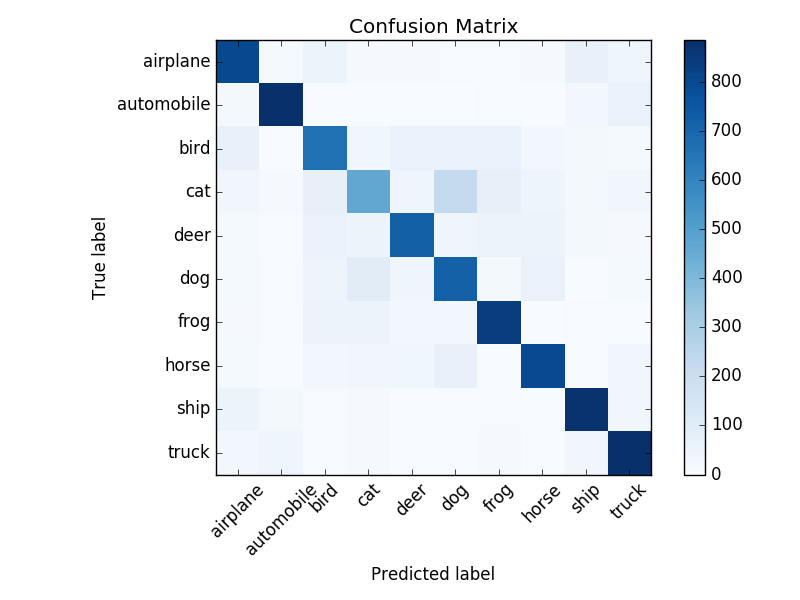
\includegraphics[width=0.45\linewidth]{8-8-14-14-3x3-15pct-color_confusion_matrix} &   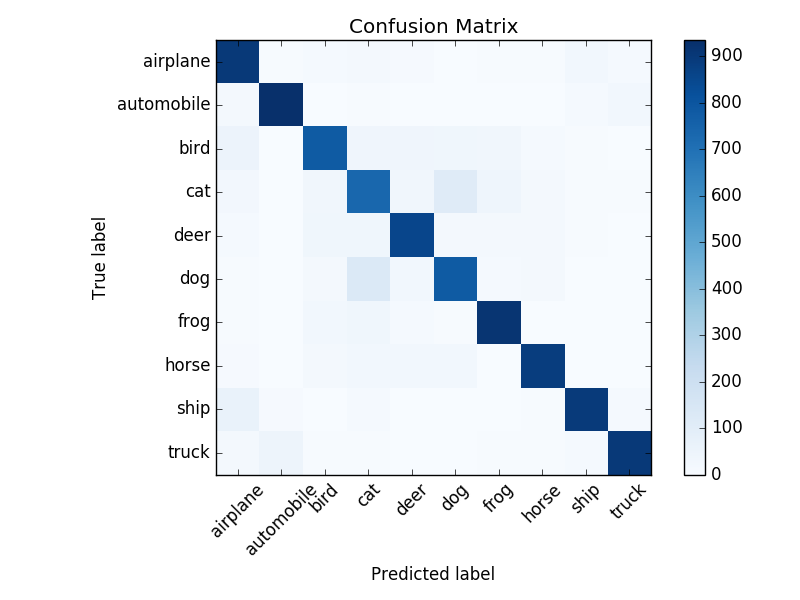
\includegraphics[width=0.45\linewidth]{24-24-48-48-3x3-15pct-color_confusion_matrix} \\
		(a) 8-8-14-14 & (b) 24-24-32-32 \\[6pt]
		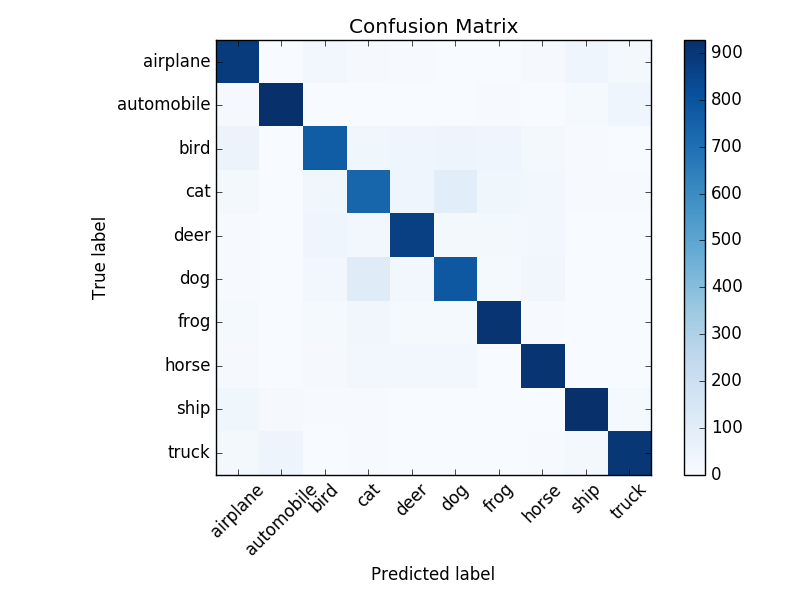
\includegraphics[width=0.45\linewidth]{32-32-64-64-3x3-15pct-color_confusion_matrix} &   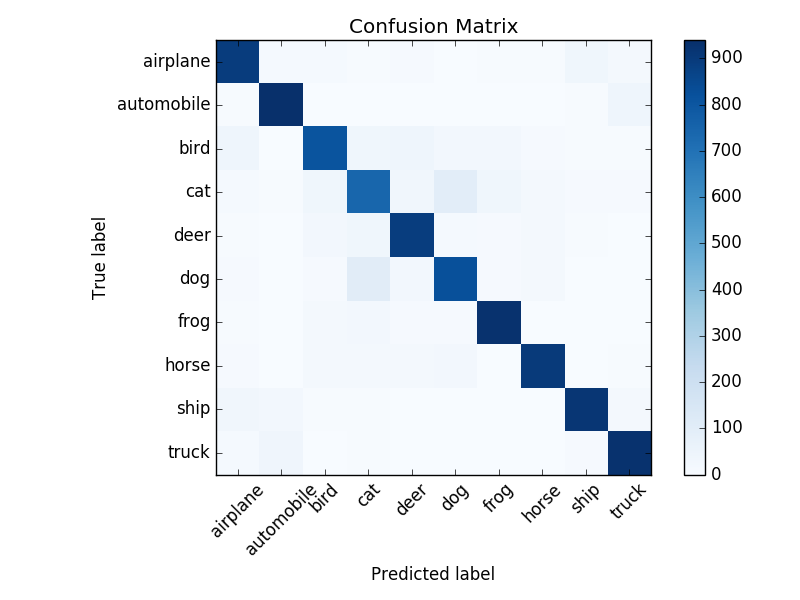
\includegraphics[width=0.45\linewidth]{48-48-96-96-3x3-15pct-color_confusion_matrix} \\
		(c) 32-32-64-64 & (d) 48-48-96-96 \\[6pt]
		\multicolumn{2}{c}{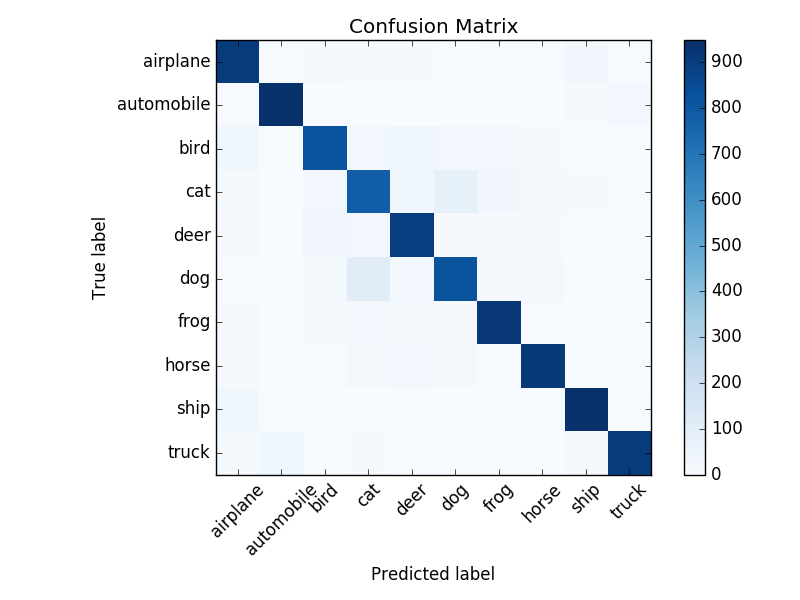
\includegraphics[width=0.45\linewidth]{128-128-256-256-3x3-15pct-no-strides-color_confusion_matrix} }\\
		\multicolumn{2}{c}{(e) 128-128-256-256}
	\end{tabular}
	\caption{Confusion Matrices varied by filter number}
	\label{confnf}
\end{figure}

As we can see from the figure \ref{confnf}, a significant improvement between out smallest model and out largest one. However it appears we hit diminishing returns after a certain number of filters as we presumably hit the limit of the features we can draw from our small 32x32 data.

From the qualification report in fig. \ref{repnf} we also see an interesting pattern we hinted on earlier in this document. Dogs and Cats are the worst performing classes with confusing happening mostly between them but dogs get confused less with cats than the opposite.

This becomes clearer when we look at the classification reports as seen in figure \ref{repnf}
\begin{figure}[h!]
	\begin{tabular}{cc}
		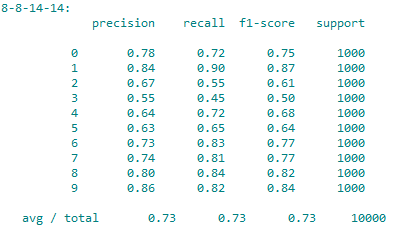
\includegraphics[width=0.45\linewidth]{8-8-14-14-3x3-15pct-color_report} &   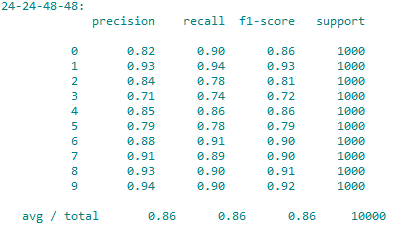
\includegraphics[width=0.45\linewidth]{24-24-48-48-3x3-15pct-color_report} \\
		(a) 8-8-14-14 & (b) 24-24-32-32 \\[6pt]
		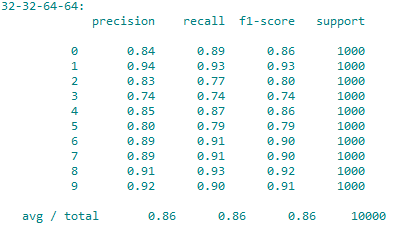
\includegraphics[width=0.45\linewidth]{32-32-64-64-3x3-15pct-color_report} &   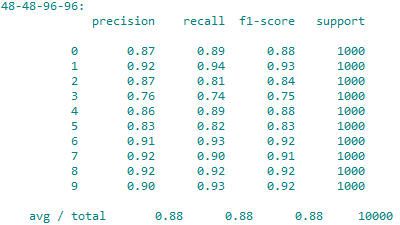
\includegraphics[width=0.45\linewidth]{48-48-96-96-3x3-15pct-color_report} \\
		(c) 32-32-64-64 & (d) 48-48-96-96 \\[6pt]
		\multicolumn{2}{c}{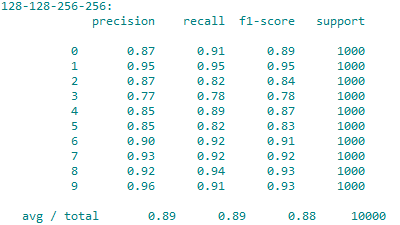
\includegraphics[width=0.45\linewidth]{128-128-256-256-3x3-15pct-no-strides-color_report} }\\
		\multicolumn{2}{c}{(e) 128-128-256-256}
	\end{tabular}
\caption{Classification Reports for experiments}
\label{repnf}
\end{figure}

As you might notice from the figures above we stop seeing overall improvements at 48-48-96-96 with small improvement in some classes, but the extra cost of the larger networks makes it a good compromise for further experiments.

\subsubsection{Effects on Size of Weights}
This investigation is much simpler. We look at the sizes of the weights we store for each network and try to correlate it the number of calculations and network complexity.

\begin{figure}[h!]
	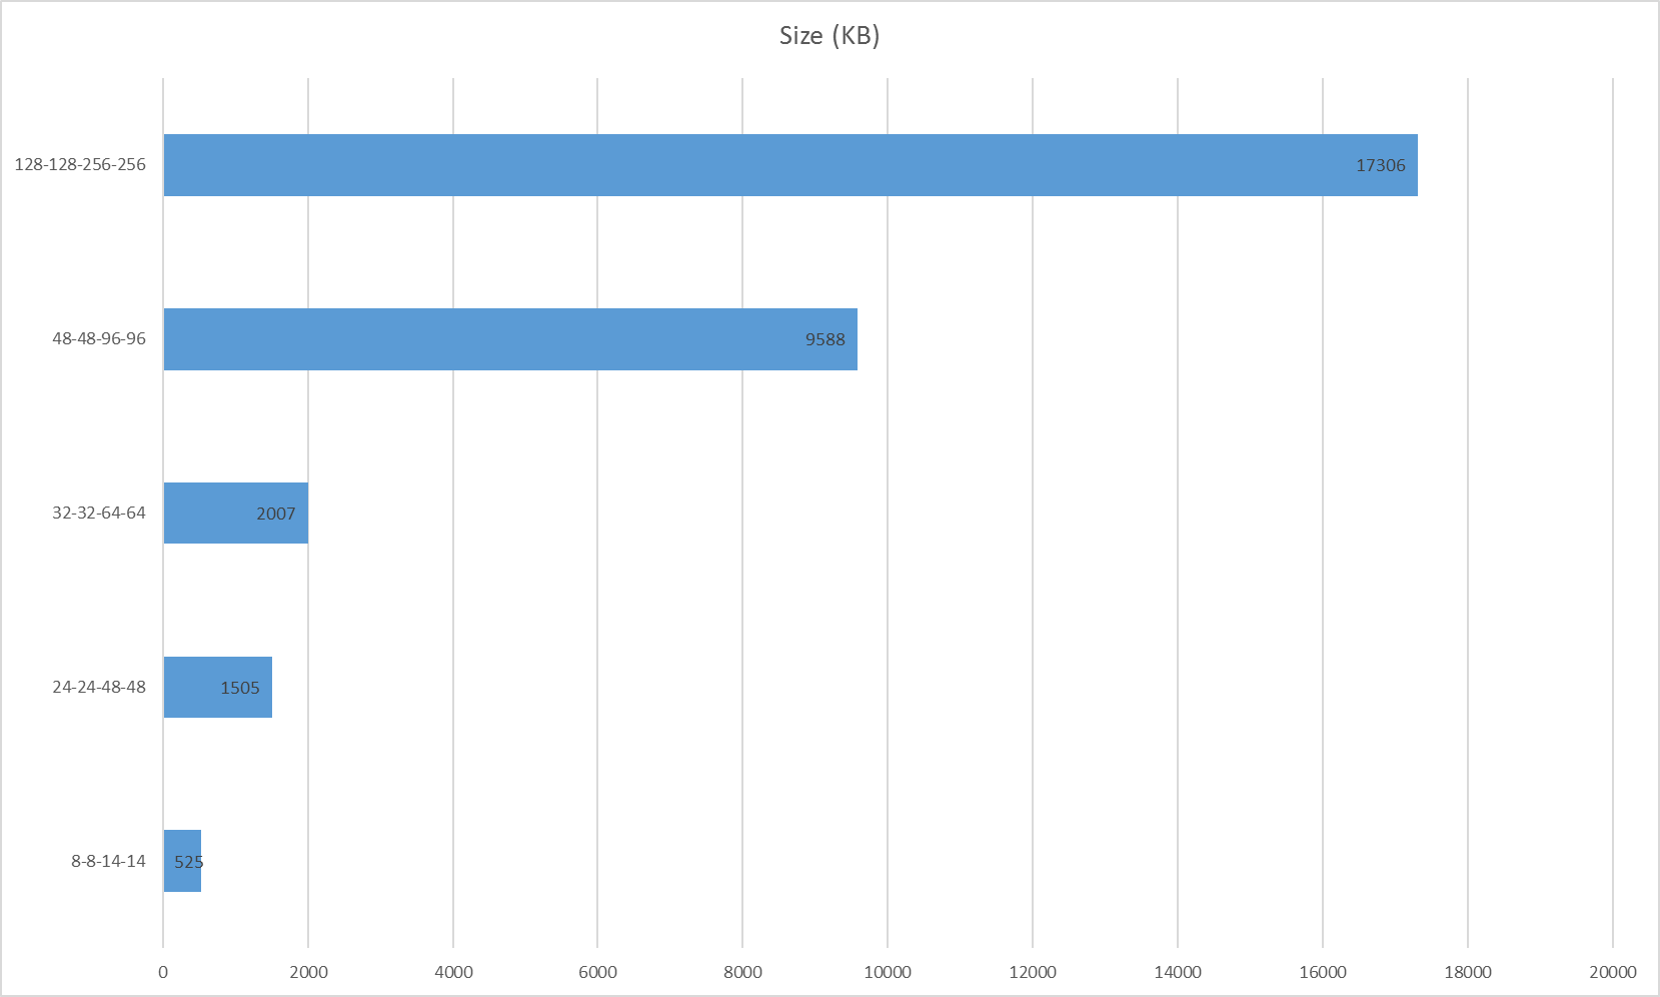
\includegraphics[width=0.8\linewidth]{datasizes_filters}
	\caption{Bar Chart of Size of Stored Weights}
	\label{sownf}
\end{figure}

In figure \ref{sownf} we can see how size increases with  more features. This makes sense since our feature maps become larger, while we can also see the increase is not completely linear with the number of neurons. This is because in CNNs weights are shared.

\subsubsection{Conclusion}
As we increase the number of our filters, we see an increase in classification performance. This comes at the expense of the simplicity of our model which impacts the speed of training, the size of the model and works as a trade-off with our classification performance.  Because of the huge cost of models larger than the 48 and the small gains we will investigate using 48 filters in situations where we are testing other hyper parameters.

\subsection{Size of Filters}
For this series of experiments we will report on the results of varying our 48-48-96-96 and 8-8-14-14 with a set of filter sizes:

\begin{itemize}
	\item 3x3
	\item 4x4
	\item 5x5
\end{itemize}

As before we are keeping all other hyper parameters the same.

\subsubsection{Effects on Training Speed}
For this we found training speed was not really affected by using larger filters in fact it was faster in some cases. We originally run this study on most of our studies but for brevity we will only look at the two extremes combinations.

\subsubsection{Effects on Performance}
We expected to see better performance with larger filters that were less numerous on account of potentially capturing larger features. Instead what we saw in fig. \ref{conffs}

\begin{figure}[h!]
	\begin{tabular}{cc}
		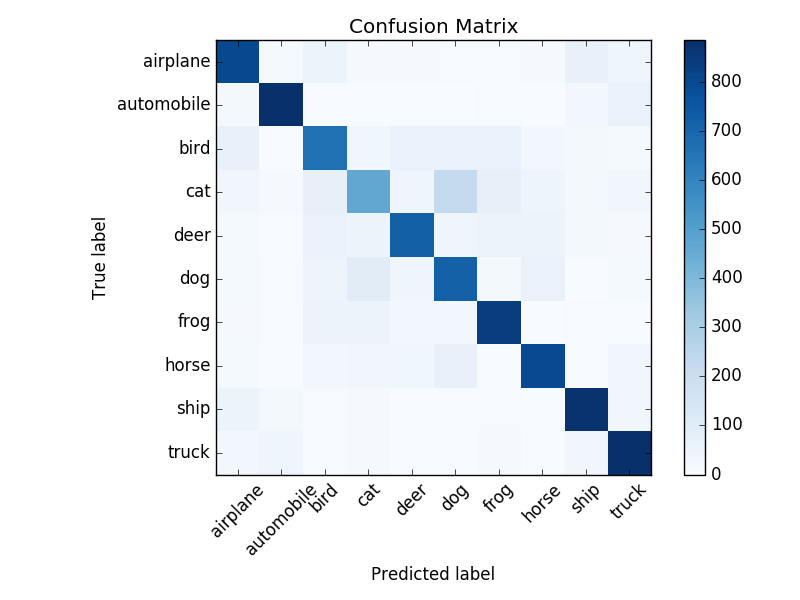
\includegraphics[width=0.45\linewidth]{8-8-14-14-3x3-15pct-color_confusion_matrix} &   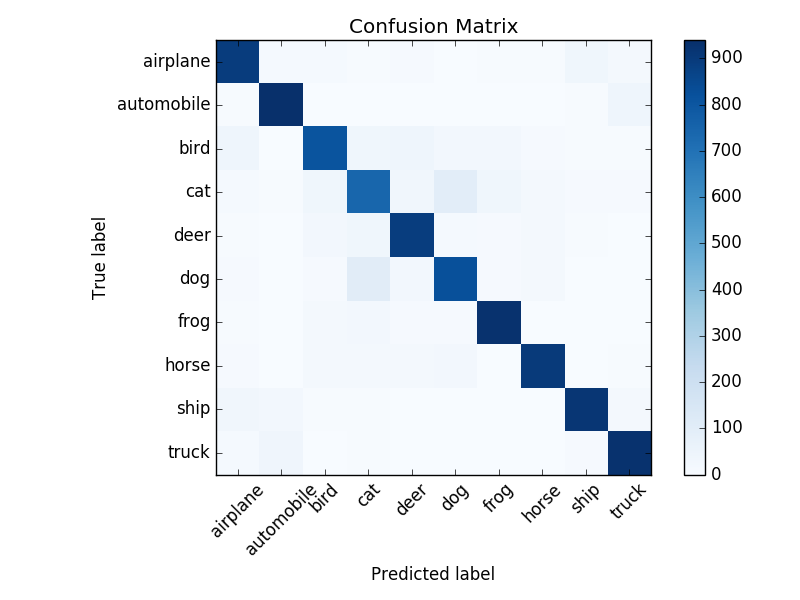
\includegraphics[width=0.45\linewidth]{48-48-96-96-3x3-15pct-color_confusion_matrix} \\
		(a) 8-8-14-14 3x3& (b) 48-48-96-96 3x3\\[6pt]
		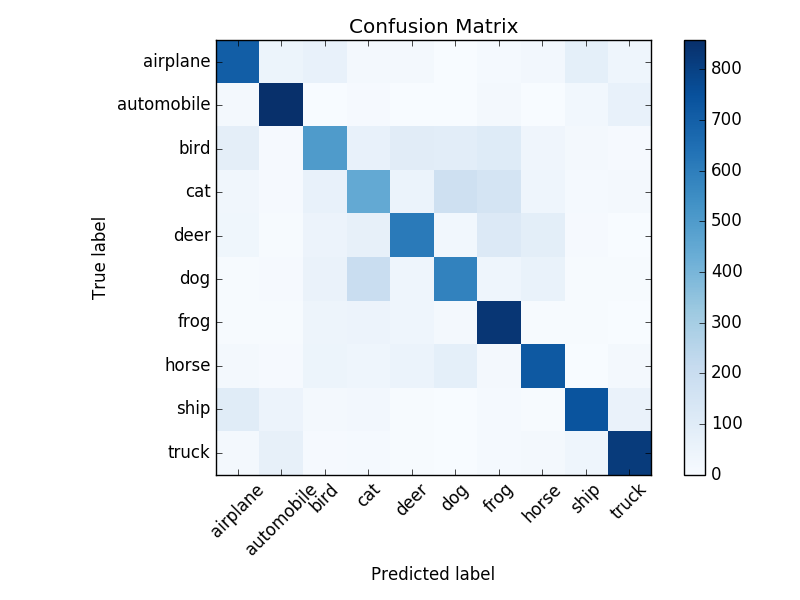
\includegraphics[width=0.45\linewidth]{8-8-14-14-4x4-15pct-no-strides-color_confusion_matrix} &   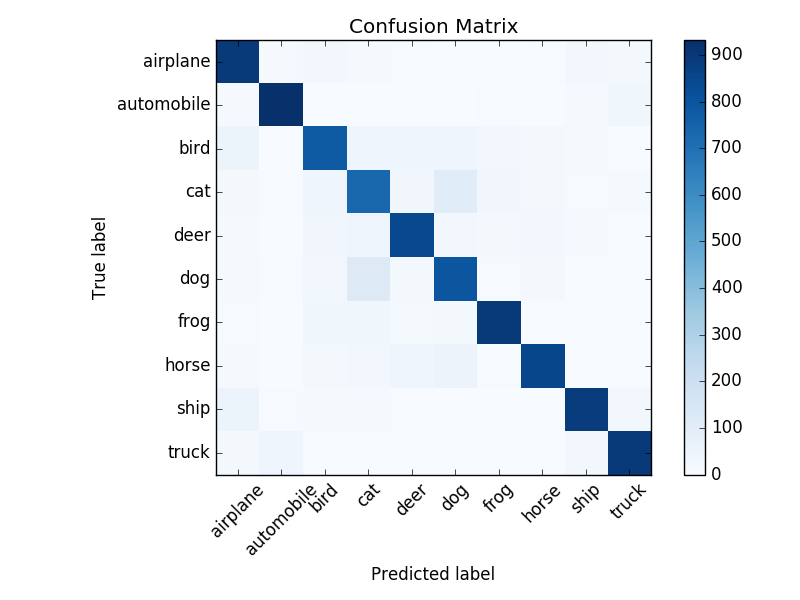
\includegraphics[width=0.45\linewidth]{48-48-96-96-4x4-15pct-no-strides-color_confusion_matrix} \\
		(a) 8-8-14-14 4x4& (b) 48-48-96-96 4x4\\[6pt]
		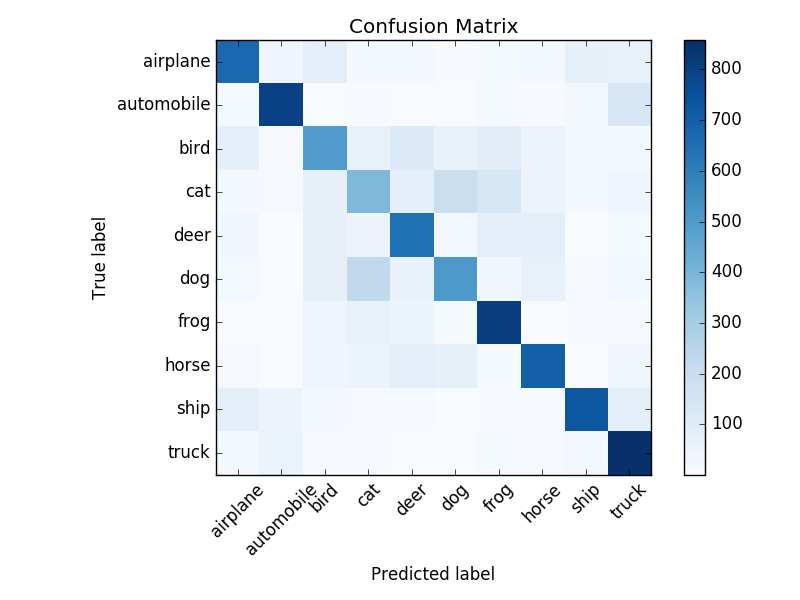
\includegraphics[width=0.45\linewidth]{8-8-14-14-5x5-15pct-no-strides-color_confusion_matrix} &   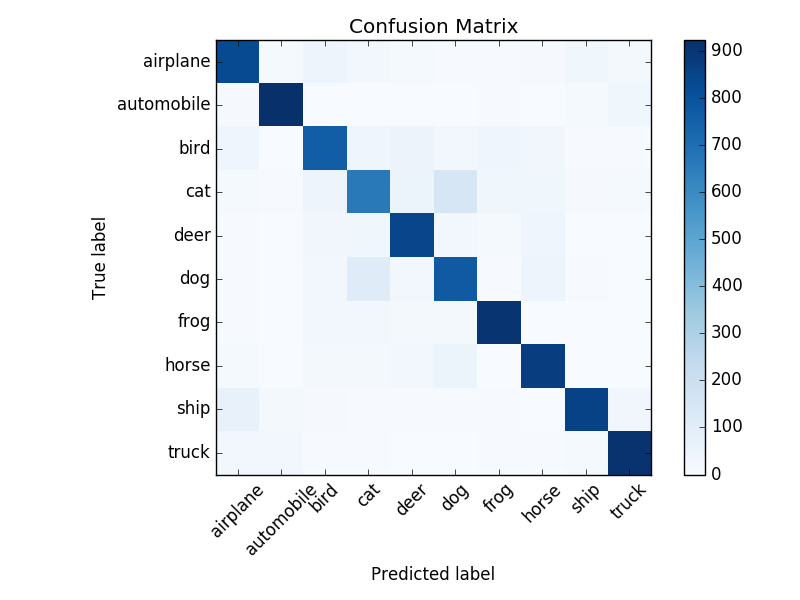
\includegraphics[width=0.45\linewidth]{48-48-96-96-5x5-15pct-no-strides-color_confusion_matrix} \\
		(a) 8-8-14-14 5x5& (b) 48-48-96-96 5x5\\[6pt]
	\end{tabular}
	\caption{Confusion Matrices varied by filter size}
	\label{conffs}
\end{figure}

We can see from the confusion matrices above that larger filters affect results negatively. The difference is so significant it can clearly be seen on the confusion matrices for smaller numbers of filters which is the opposite than what we initially expected.

The other pattern we observe is filter numbers still matter with larger filters we see an improvement in the 48 model. However they never match the smaller filters though the results do converge somewhat.

We believe this might be worse due to the nature of our training images. Remember the images are quite small at 3x3. This also means that any feature in those images is also going to be very small. As a result many small filters seem to be the way to go here.

Due to how significant the difference is we will not be adding the classification report but we note a range of accuracy of 0.60 to 82 on the smaller network.
\subsubsection{Effects on Size of Weights}

\subsubsection{Conclusion}
Larger filters are not really advisable in this dataset as they give no real practical benefits over 3x3 filters in performance, and training speed. Size of weights does not mitigate the loss in classification performance.

\subsection{Augmentation}
For this section we will only use the 48 network again. As a consistent good performer, and having seen the performance of 3x3 networks with 2 layers between max pooling in this dataset we use it as our reference.

For our augmentation we decided to use a rotation range of 0.1, a horizontal and vertical shift range of 0.8 and a random horizontal flip here. From the intelligence we have in our data and smaller experiments these should work well.
\subsubsection{Effects on Training Speed}
Here we saw very significant drops in speed. This is largely because augmentations need to run  on each batch and run on a single CPU thread. This means that we are bottlenecked by the CPU as the GPU idles waiting for images to train on. One way we observe this is that models are restricted to a minimum of 12s per epoch with it on with no decrease in this time despite trying out parameters that helped in the past.

This could be alleviated if Keras used a parallel image augmentation mechanism since this problem can be solved in a divide a conquer algorithm. We lose about 50-80 percent per epoch to this, impact also depends on the number of channels. Because of this we'll be looking at the benefits both in colour and greyscale.

\subsubsection{Effects on Overfitting}
We would like to see how quickly our model overfits. If our Augmentation works we expect to see a significant reduction in overfitting that should in theory increase our classification performance
\begin{figure}[h!]
	\begin{tabular}{cc}
		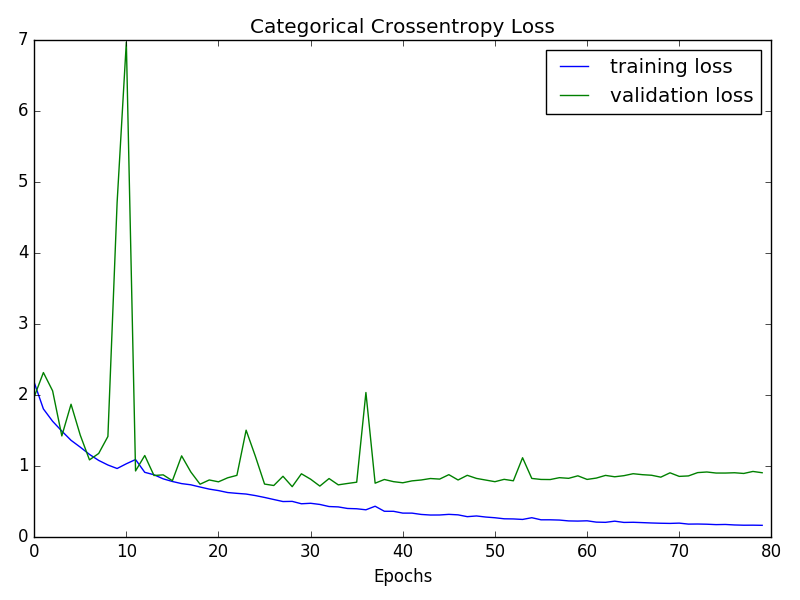
\includegraphics[width=0.45\linewidth]{48-48-96-96-15pct-no-strides-no_aug_learning_rate} &   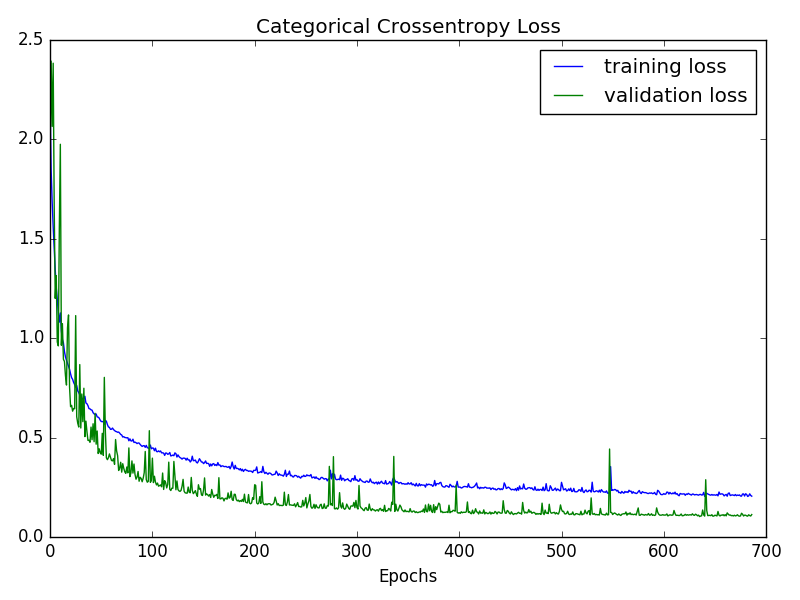
\includegraphics[width=0.45\linewidth]{48-48-96-96-15pct-no-strides_learning_rate} \\
		(a) 1 channel no augmentation & (b) 1 channel augmentation \\[6pt]
		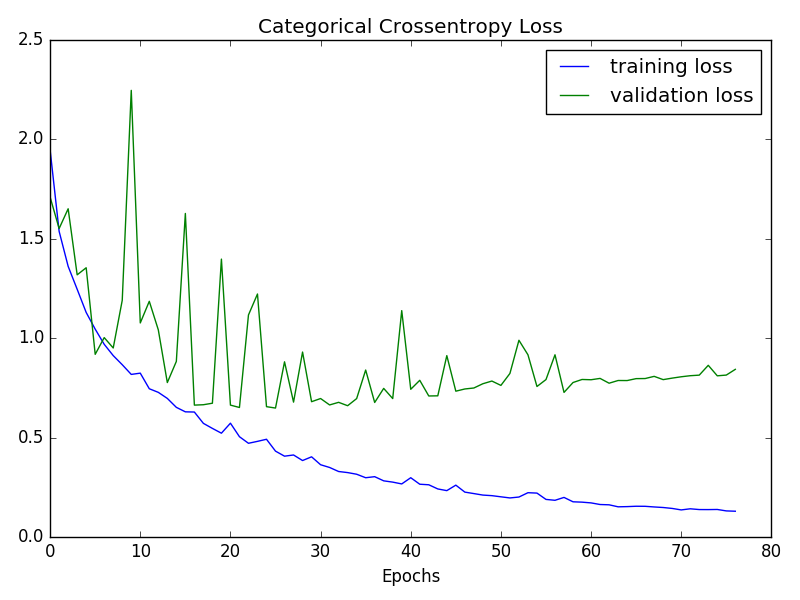
\includegraphics[width=0.45\linewidth]{48-48-96-96-15pct-no-strides-color-no_aug_learning_rate} &   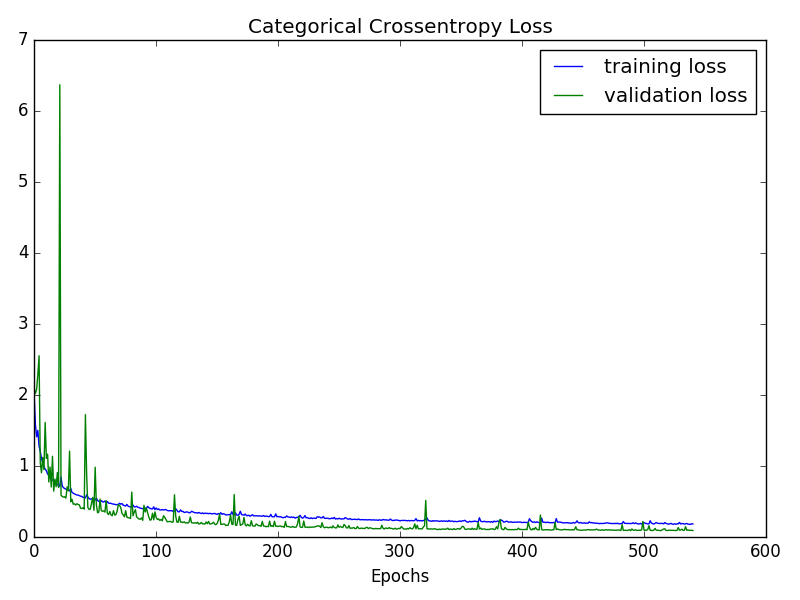
\includegraphics[width=0.45\linewidth]{48-48-96-96-15pct-no-strides-color_learning_rate} \\
		(c) 3 channels no augmentation & (d) 3 channel augmentation \\[6pt]
	\end{tabular}
	\caption{Plot of Training History in Terms of Loss}
\end{figure}

As we can see in the figure, we are seeing a surprisingly significant improvement in our cross-validation results. With a patience of 50, we end up terminating at close to 80 epochs without augmentation. This should reflect very negatively in our generalised classification performance.

An observant reader might also notice local minima for validation loss that is consistent with what we'd expect to see and the main reason we use Early Stopping.
\subsubsection{Effects on Performance}
Following our earlier results we are eager to see whether there is any impact and if so what is it with not using augmentation in terms of results. We've seen it leads to very fast overfitting but does this translate to results?
\begin{figure}[h!]
	\begin{tabular}{cc}
		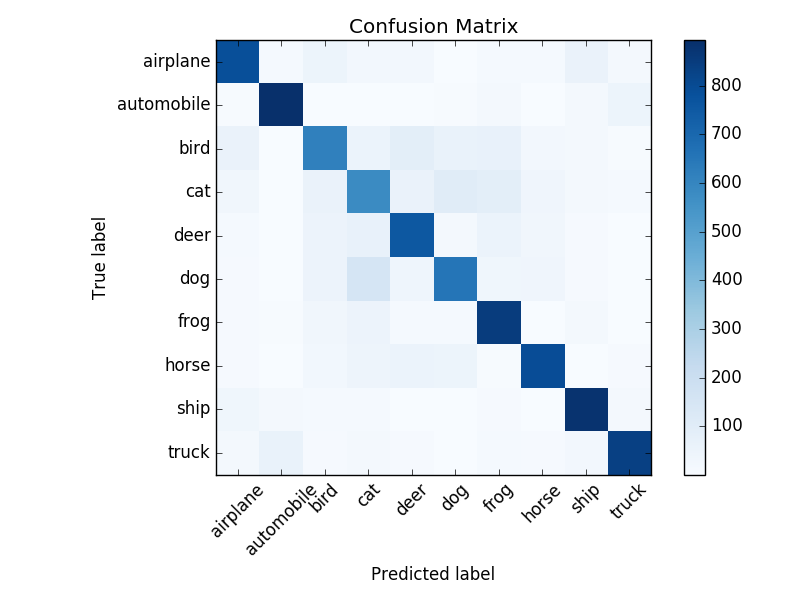
\includegraphics[width=0.45\linewidth]{48-48-96-96-15pct-no-strides-no_aug_confusion_matrix} &   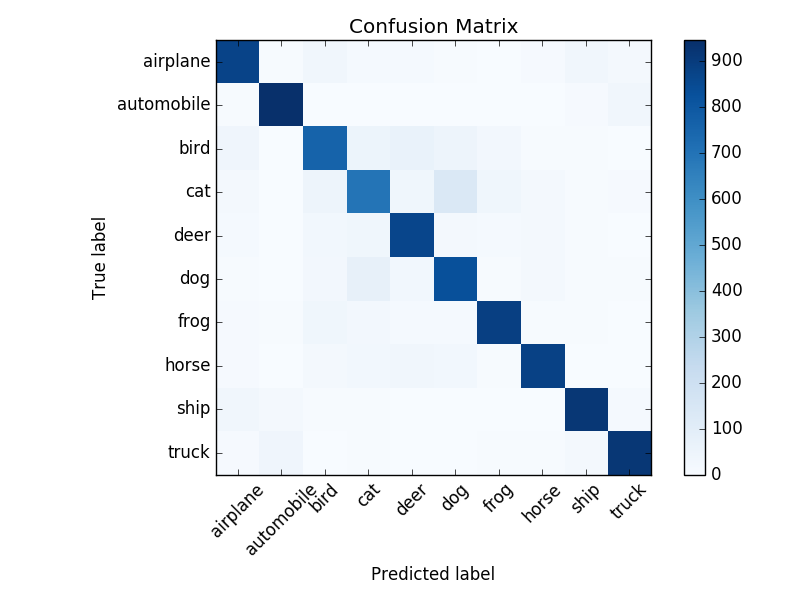
\includegraphics[width=0.45\linewidth]{48-48-96-96-15pct-no-strides_confusion_matrix} \\
		(a) 1 channel no augmentation & (b) 1 channel augmentation \\[6pt]
		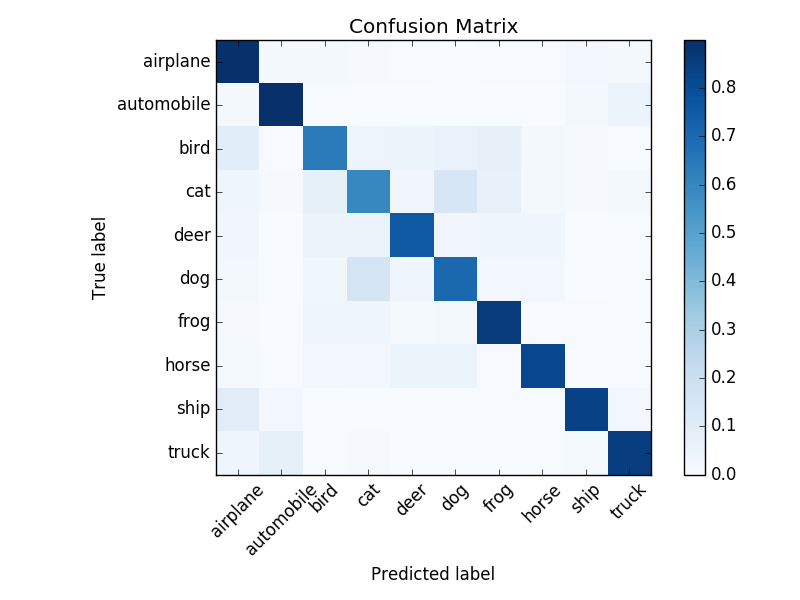
\includegraphics[width=0.45\linewidth]{48-48-96-96-15pct-no-strides-color-no_aug_confusion_matrix} &   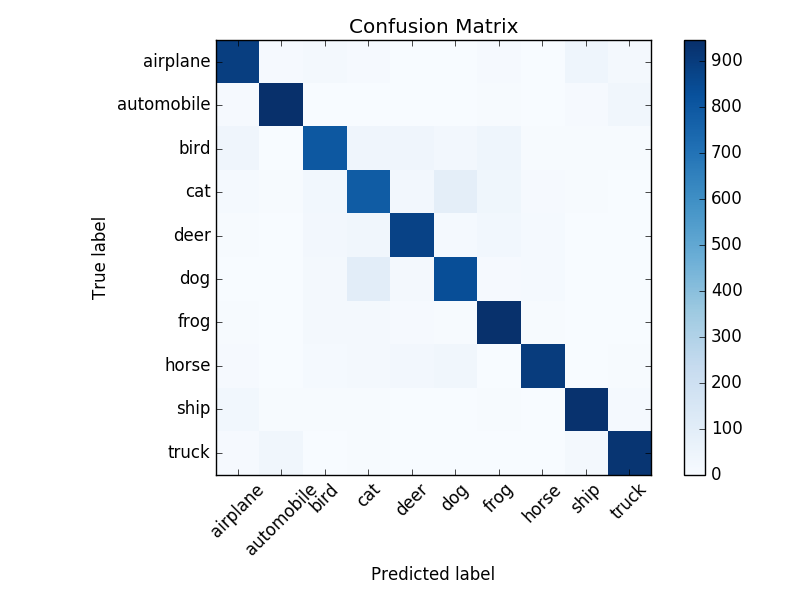
\includegraphics[width=0.45\linewidth]{48-48-96-96-15pct-no-strides-color_confusion_matrix} \\
		(c) 3 channels no augmentation & (d) 3 channel augmentation \\[6pt]
	\end{tabular}
	\caption{Confusion Matrices for Augmentation Experiment}
\end{figure}

We can see just from the confusion matrix that performance takes a big hit without our augmentation. Indeed looking at our f1 score in the reports we can see 0.76 and 0.86 between the two options in greyscale. A very significant difference.

Looking very briefly at older logs from past experiments we also notice a pattern that larger networks tend to benefit more from augmentation. To corroborate our results we re-run the experiment:

\begin{figure}[h!]
	\begin{tabular}{cc}
		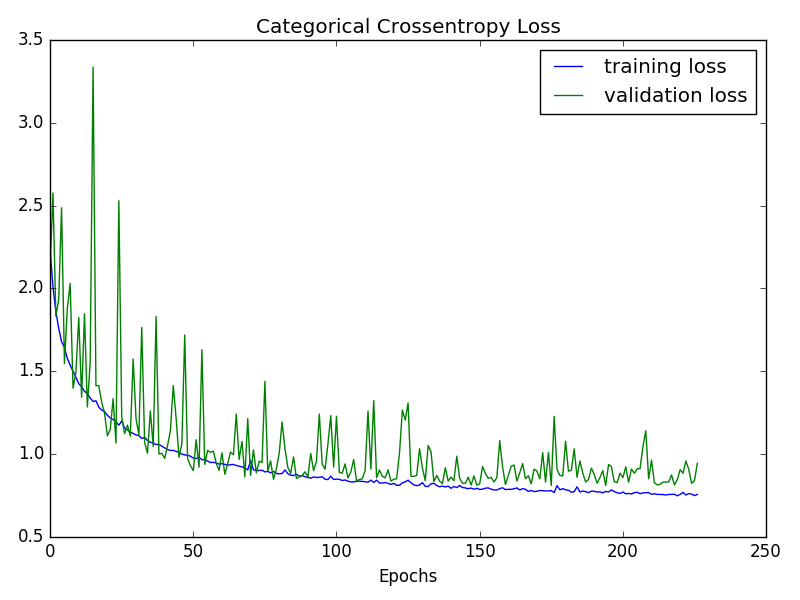
\includegraphics[width=0.45\linewidth]{8-8-14-14-15pct-no-strides-no_aug_learning_rate} &   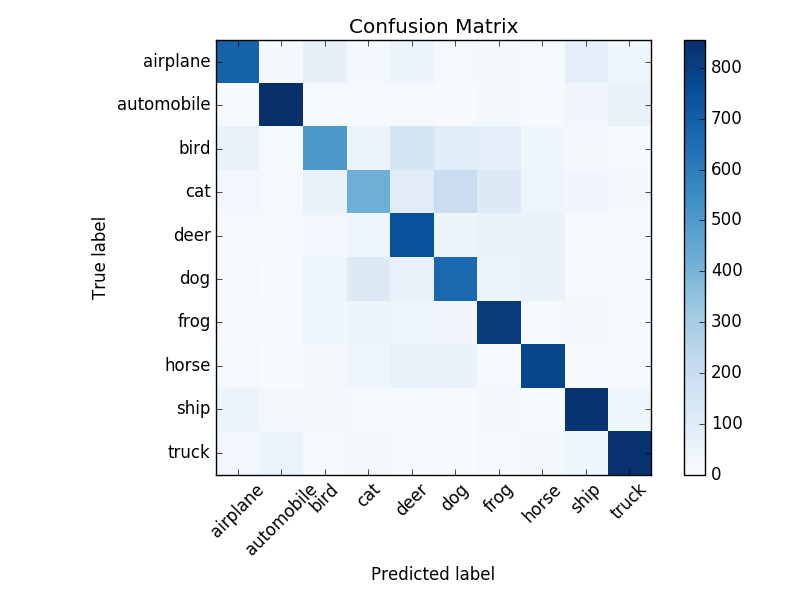
\includegraphics[width=0.45\linewidth]{8-8-14-14-15pct-no-strides-no_aug_confusion_matrix} \\
	\end{tabular}
	\caption{Small model with 8-8-14-14 3x3 filters no augmentation}
\end{figure}

\subsection{Conclusions}
Data augmentation helps significantly to reduce overfitting and improve performance in our models. The performance cost is very significant with the current implementation of it but results benefit enough that it would be foolish not to use it.

If also appears that the larger the network the more important good augmentation becomes. This makes some sense as with more features extracted, our network would be increasingly likely to overfit so avoiding this is important.

\subsection{Number of Colour Channels}
\subsubsection{Effects on Training Speed}
Going from our augmentation results we are eager to observer how colour affects the training speed. We use the 48 as usual as our reference. Conversion takes some extra time especially on our Mode 4 conversion method. What we see however is a big boost in speed. This makes sense since we reduce inputs to a third which means there is much less processing to do.

The effect is more pronounced when augmentation is used where the performance gap widens. Presumably this is because there is much less data to convert which reduces CPU cost for the augmentation code.
\subsubsection{Effects on Performance}
\subsubsection{Effects on Size of Weights}
Minimal increases in the size of the weights was observed here. This is because with a CNN weights are shared by neurons, for the colour that's especially handy as it makes a 3x increase in inputs have a very negligible impact in size.

\subsection{Multi Layer Perceptron: Figures in Matrices}
As an early test we obtained a number of results from MLPs. Here we have collated some of the most interesting ones showing the effects of depth of MLPs in terms of training and classification performance

\section{Miscellaneous Discussion}
\subsection{Accounts of Early Experiments}
Here we will discuss the earliest parts of our experimentation. These were done before the experimental infastructure was complete so we don't have complete figures recorded for them. These accounts are based on logs and diary entries taken at the time. Rapid prototyping was taking place at the time so results might not be consistent. As a result this section is included in a pure discussion format and is aimed to offer some insight to early decisions taken in this project.

\subsubsection{Early Experiments}
Early on we experimented with decay, momentum, activation functions and learning rate. We ended up finding that defaults or near defaults for these values worked well for our training solution so we left them as is for the final results in an effort to reduce the hyperparameters we reported on.


\subsection{Conclusion}
From our experiments we learned a number of things about CNN design for this set. First lesson was that larger models can get higher results but suffer from diminishing returns and overfitting.

A successful model for this dataset needs a good augmentation strategy, more aggressive augmentation works to an effect but it is important to try to maintain as many features as possible to maintain performance. Features are small so one needs to moreso careful.

Colour gives a small bump but experimenting in greyscale can give significant speed improvements which makes optimisation go much quicker since we can get results faster. Ideally we can only switch to colour for final results.

Larger filters are generally not very good for this dataset. Features are quite fine so 3x3 seems to work quite well from all our experiments and benefits of other filters seem lacklustre from our experiences.

Deeper networks can do well in this dataset and deal better with more aggressive augmentation but the size of the CNN seems to be more important. Very deep networks are hard to train with random initialisation so require different strategies to take advantage of. We did not have time to properly test implications for this.

From looking at these results we can also conclude that for some problems, neural networks might be reasonable ready to be sold, with accuracies exceeding 88 percent for a small student project.